
\chapter{Kap København}
\label{appendix:kapk}

The following pages contain the paper published in Nature 2022:

\begin{quote}
    Kurt H. Kjær, Mikkel W. Pedersen, Bianca De Sanctis, Binia De Cahsan, Thorfinn S. Korneliussen, \textbf{Christian Michelsen}, Karina K. Sand, Stanislav Jelavić, Anthony H. Ruter, Astrid M. Z. Bonde, Kristian K. Kjeldsen, Alexey S. Tesakov, Ian Snowball, John C. Gosse, Inger G. Alsos, Yucheng Wang, Christoph Dockter, Magnus Rasmussen, Morten E. Jørgensen, Birgitte Skadhauge, Ana Prohaska, Jeppe Å. Kristensen, Morten Bjerager, Morten E. Allentoft, Eric Coissac, PhyloNorway Consortium, Alexandra Rouillard, Alexandra Simakova, Antonio Fernandez-Guerra, Chris Bowler, Marc Macias-Fauria, Lasse Vinner, John J. Welch, Alan J. Hidy, Martin Sikora, Matthew J. Collins, Richard Durbin, Nicolaj K. Larsen \& Eske Willerslev, \emph{``A 2-million-year-old ecosystem in Greenland uncovered by environmental DNA''} (Published in Nature, 2022, doi: 10.1038/s41586-022-05453-y).
\end{quote}
The paper use the \metaDMG tool to identify ancient species and classify the amount of ancient damage in these species.  This shows, that modern modern statistical methods combined with excellent work in the ancient DNA labs can provide new insights into the past -- even on more than two millions years old data.

\clearpage
% trim={<left> <lower> <right> <upper>}
% \includepdf[scale=.7,pages=-,trim={10mm 10mm 10mm 10mm},pagecommand={}]{papers/kapk.pdf}
XXX

% - - - - - - - - - - - - - - - - - - - - - - - - - - - - - - - - - - - - - - -


\chapter{Explainable ML and Anaemia}
\label{appendix:anaemia}

The following pages contain the draft paper:

\begin{quote}
    Christoffer C. Jørgensen, \textbf{Christian Michelsen}, Troels C. Petersen, Henrik Kehlet (2022), \emph{``Gender-specific haemoglobin thresholds in relation to preoperative risk assessment in fast-track total hip and knee arthroplasty''}.
\end{quote}
Based on the same data as used on Paper II, the paper uses the SHAP curves to understand the machine learning model. In particular, it compares the preoperative haemoglobin level in the patient with the risk-score for being resubmitted to the hospital within 30 days after the operation, stratified by sex and operation type (knee vs. hip replacement).
\clearpage
% trim={<left> <lower> <right> <upper>}
% 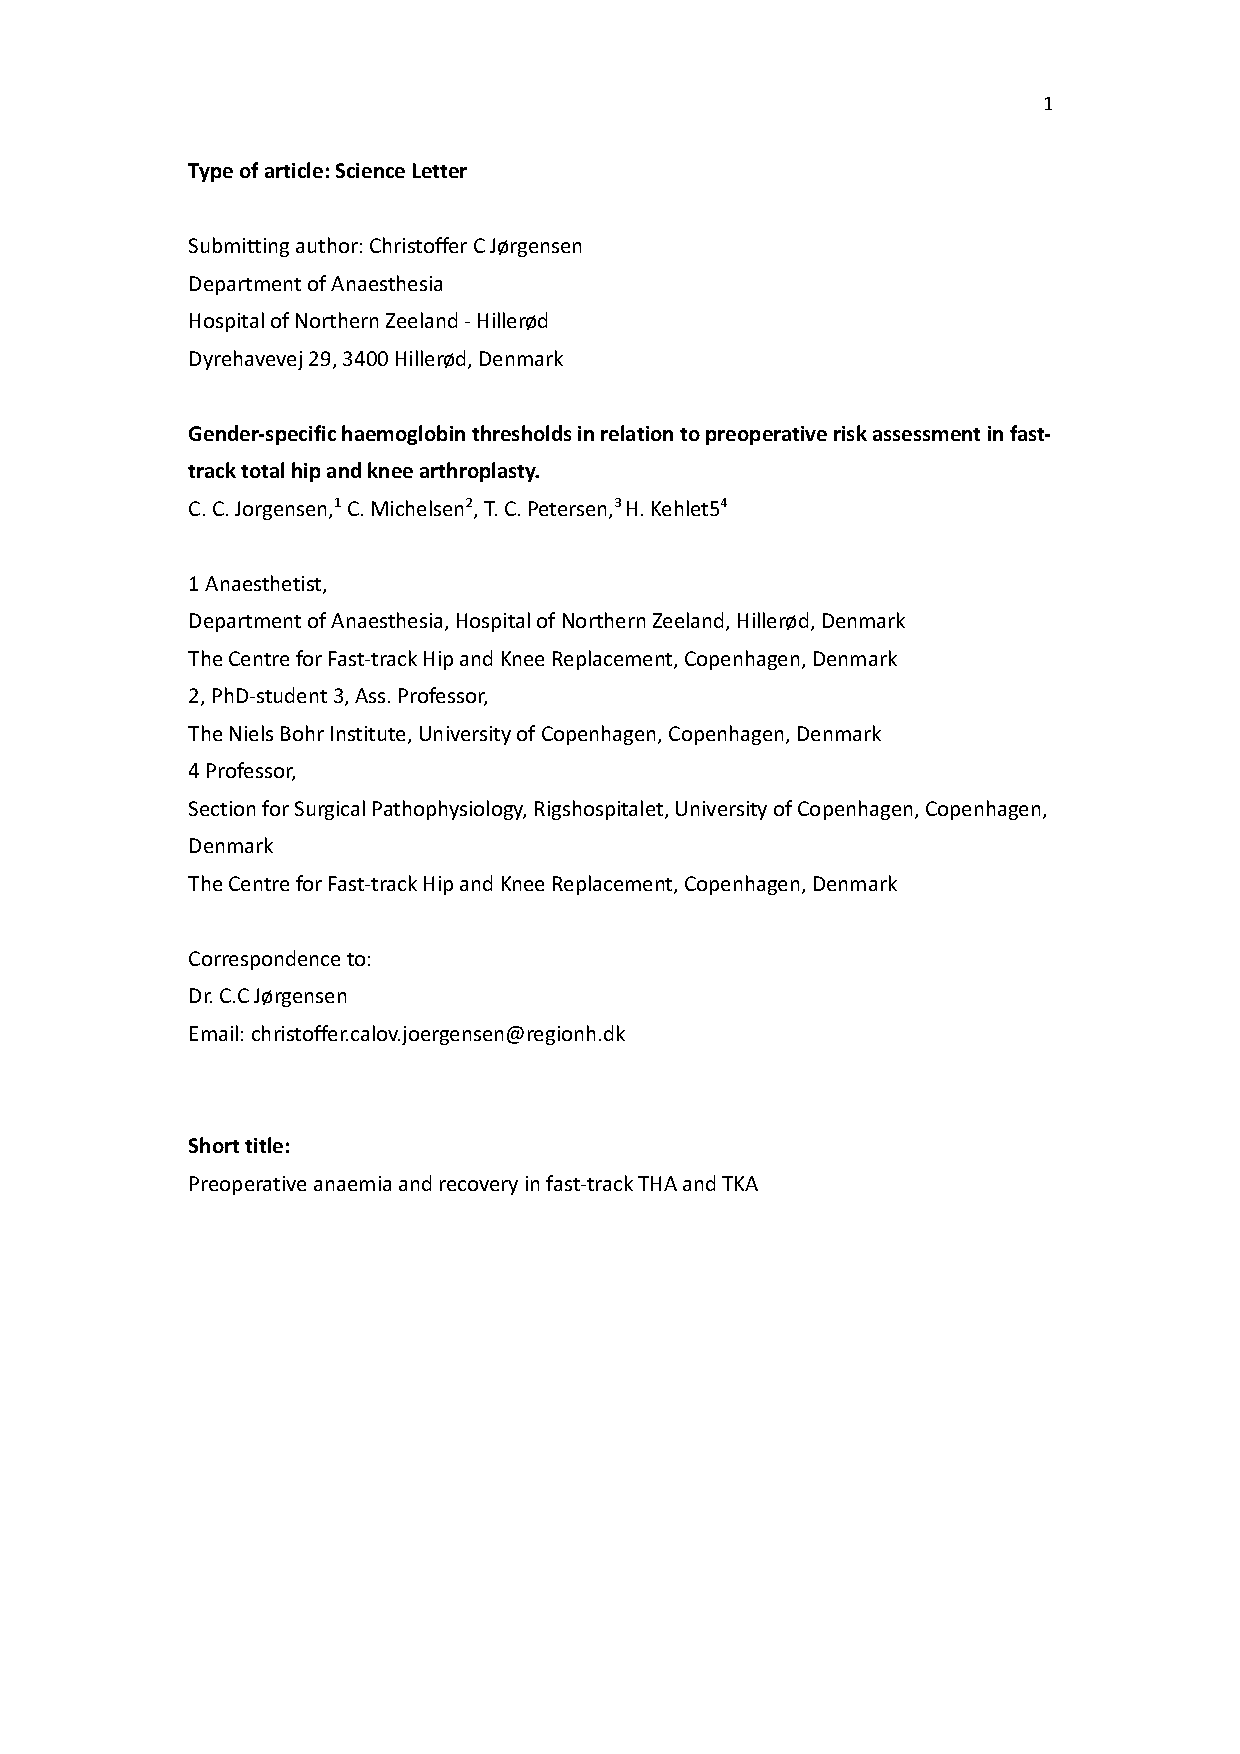
\includepdf[scale=.7,pages=-,trim={10mm 10mm 10mm 10mm},pagecommand={}]{papers/anaemia.pdf}
XXX


% - - - - - - - - - - - - - - - - - - - - - - - - - - - - - - - - - - - - - - -

\chapter{SSI Ekspertrapport}
\label{appendix:ssi-report}

The following pages contain the report from Statens Serum Institut, the Danish CDC:
\begin{quote}
    Ekspertgruppen for matematisk modellering, \emph{``Ekspertrapport af den 10. december 2020 -- Effekten af kontaktopsporing''} (Statens Serum Institut, 2020).
\end{quote}
The report is from December 10, 2020 and is a summary on the effect of contact tracing related to COVID-19 in Denmark. The report is in Danish and is based on two agent based models, one from DTU and our model from NBI.

\clearpage
% trim={<left> <lower> <right> <upper>}
% 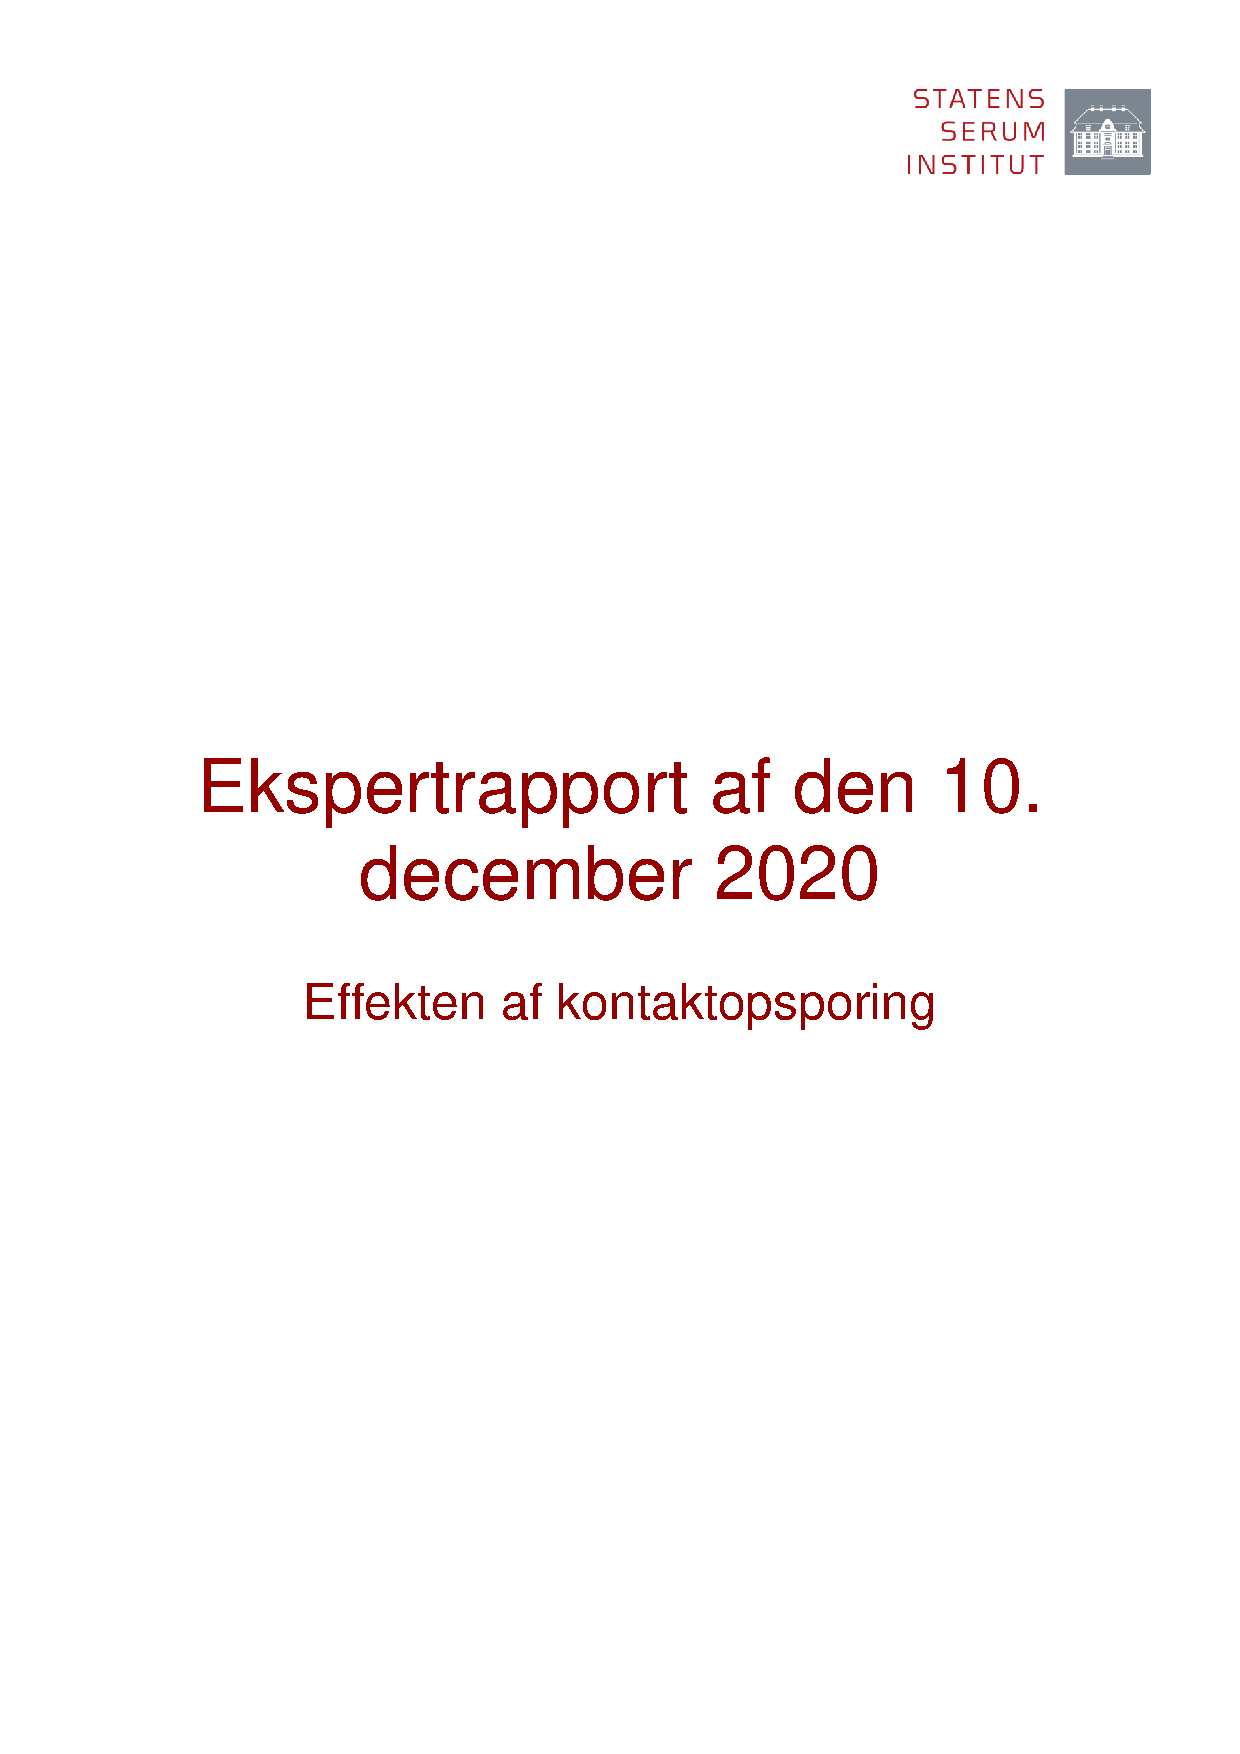
\includepdf[noautoscale,pages=-,trim={0mm 0mm 0mm 0mm}]{papers/SSI_1.pdf}
% 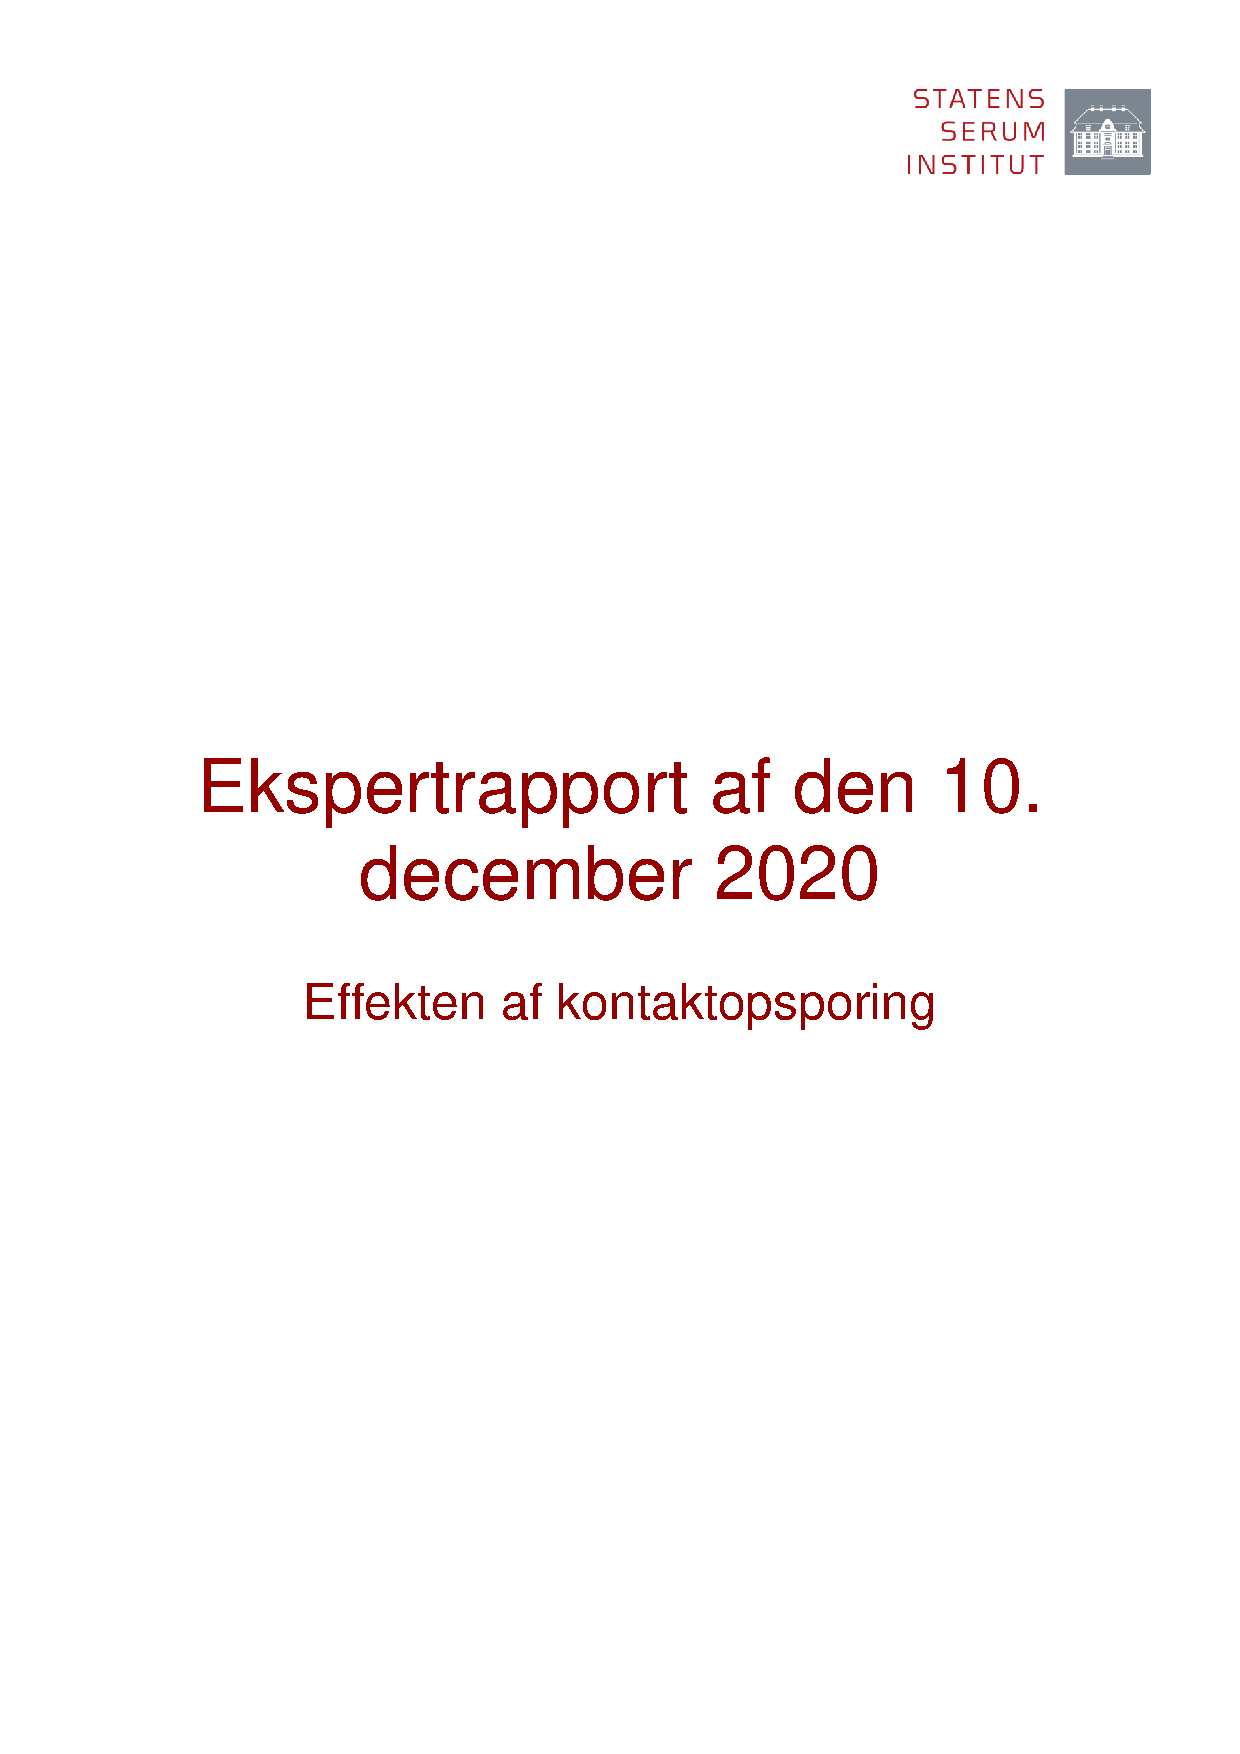
\includepdf[scale=.7,pages=-,trim={10mm 10mm 10mm 10mm},pagecommand={}]{papers/SSI_1.pdf}
XXX


% - - - - - - - - - - - - - - - - - - - - - - - - - - - - - - - - - - - - - - -

\chapter{SSI Notat}
\label{appendix:ssi-notat}

The following pages contain the report from Statens Serum Institut, the Danish CDC:
\begin{quote}
    Ekspertgruppen for matematisk modellering, \emph{``Scenarier for udviklingen i den engelske virusvariant af SARS-COV-2 (cluster B.1.1.7)''} (Statens Serum Institut, 2021).
\end{quote}
The report is from January 2, 2021 and is a summary of the estimated spread of the ``alpha'' variant of COVID-19 (B.1.1.7) in Denmark. The report is in Danish and is based on two models, one from DTU and our agent based model from NBI.

\clearpage
% trim={<left> <lower> <right> <upper>}
% 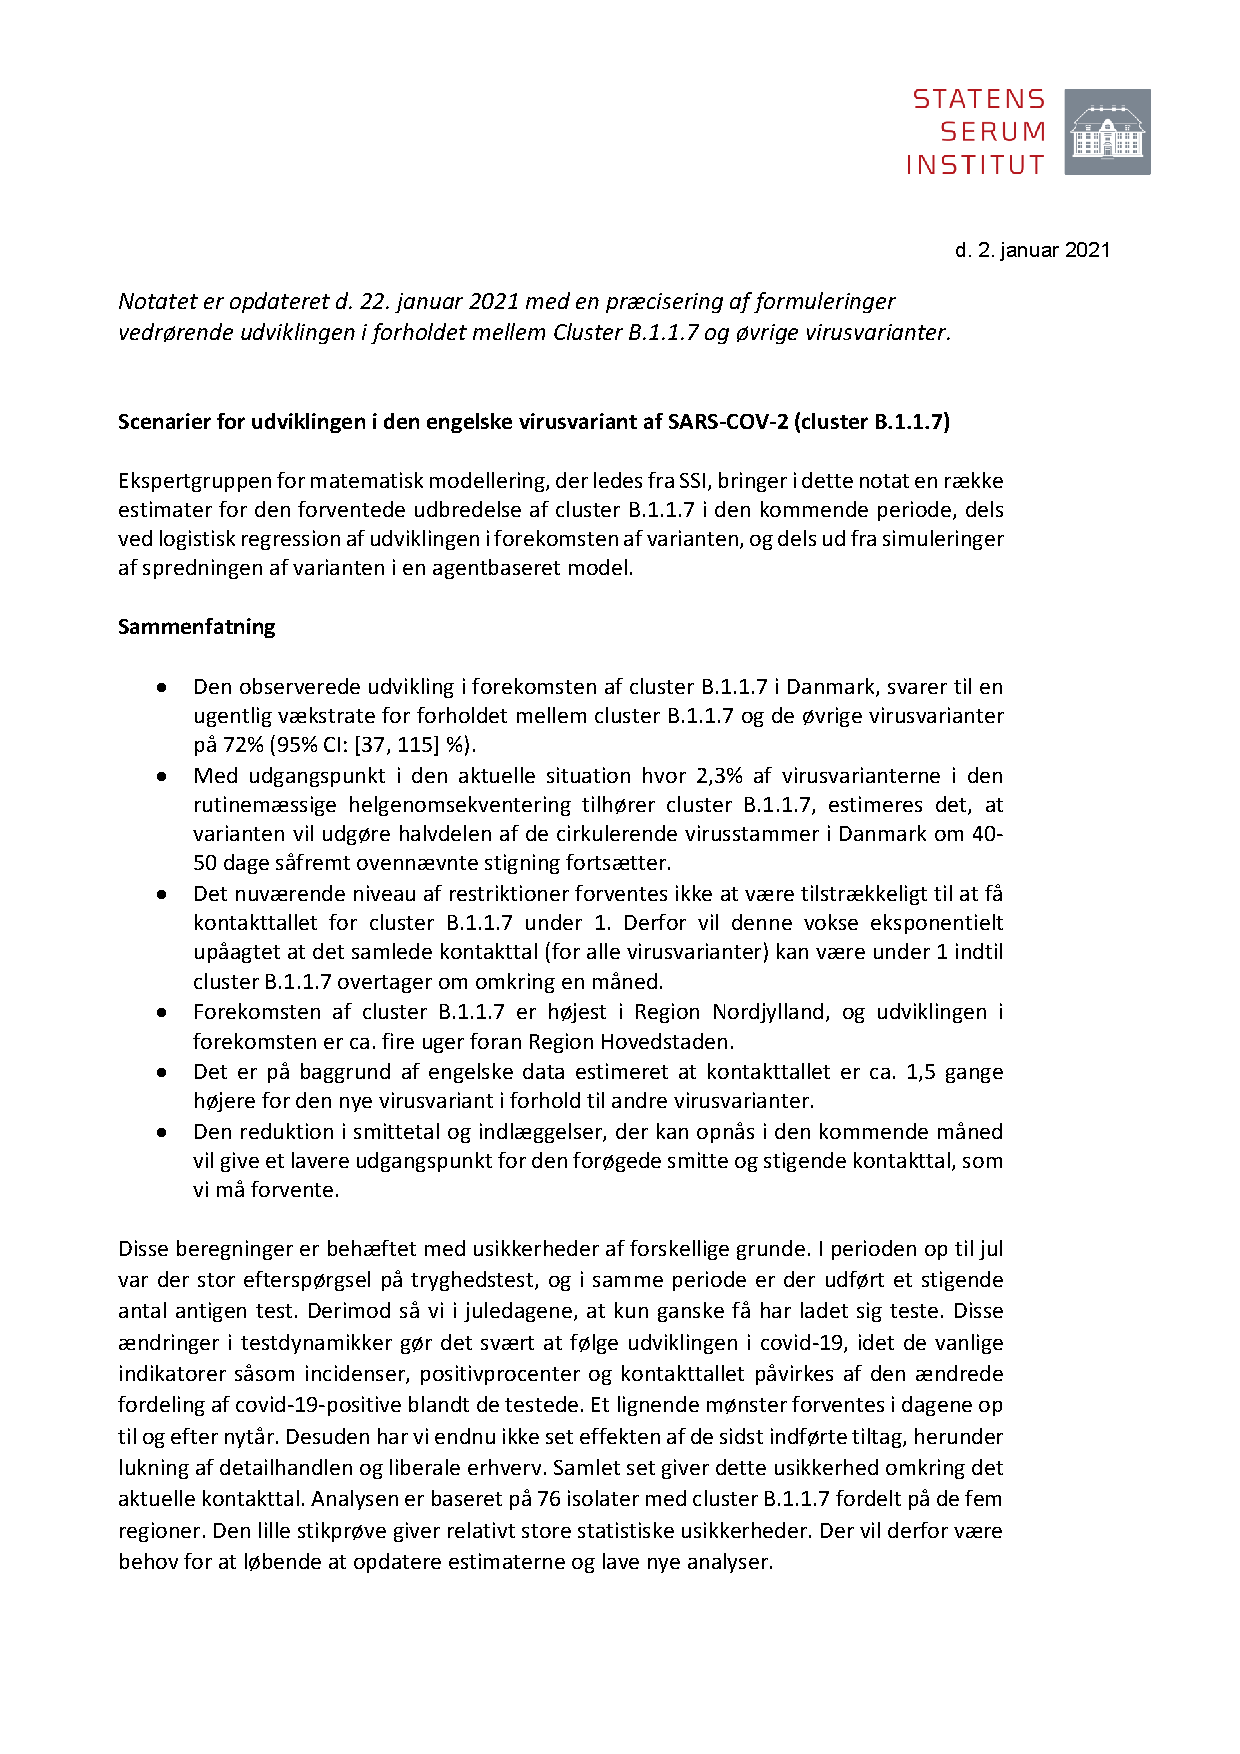
\includepdf[scale=.7,pages=-,trim={10mm 10mm 10mm 10mm},pagecommand={}]{papers/SSI_2.pdf}
XXX


